\documentclass[conference]{acmsiggraph}

\TOGonlineid{45678}
\TOGvolume{0}
\TOGnumber{0}
\TOGarticleDOI{1111111.2222222}
\TOGprojectURL{}
\TOGvideoURL{}
\TOGdataURL{}
\TOGcodeURL{}

\title{Ray Tracing Implicit Surfaces}

\author{David Rusk\thanks{e-mail:drusk@uvic.ca}\\University of Victoria}
\pdfauthor{David Rusk}

\keywords{ray tracing, implicit surfaces}

\begin{document}

\maketitle

\begin{abstract}

Write abstract here. \cite{KalraBarr1989}

\end{abstract}

\keywordlist

%% Use this only if you're preparing a technical paper to be published in the 
%% ACM 'Transactions on Graphics' journal.

\TOGlinkslist

%% Required for all content. 

\copyrightspace

\section{Introduction}

Write introduction here.

\section{Background}

Write background here.

\section{Methodology}

Write methodology here.

\section{User Interface}

Write interface description here.

\section{Data Structures}

Write data structures description here.

\section{Algorithms}

Write algorithms description here.

\section{Implementation}

There are many open source ray tracers available on the internet.  However, 
for pedagogical reasons it was decided to implement a simple ray tracer from 
scratch.  This also made it easier to modify and adapt to support implicit
surfaces because many of the open source ray tracers are part of larger 
packages or have a lot of additional functionality.

The implementation was done in C++ and used no external libraries.  Output 
images were written to PPM \cite{PPM} files because the PPM format is 
very simple and can be implemented trivially without external libraries.

The project source code is available online at 
https://github.com/drusk/ImplicitRayTracer

\section{Results}

The system developed can currently render spheres with adjustable locations,
radii, colours, reflectivity and transparency.  The below figure shows a
simple example.  The ground is made using a sphere with a very large radius.
The light source (not in the field of view) is also a sphere.  Except for the
ground sphere, all of them are reflective.  Only the green sphere has some
transparency.

\begin{figure}[ht]
  \centering
  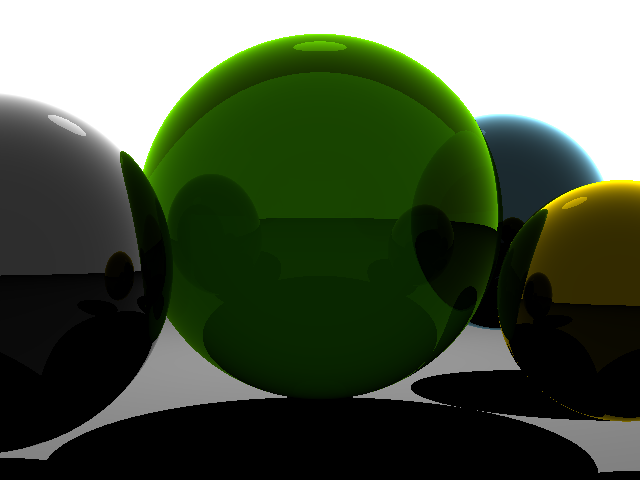
\includegraphics[width=1.5in]{figures/spheres.png}
  \caption{Example of ray traced spheres.}
\end{figure}

\section{Conclusion}

Write conclusion here.

\section{Future Work}

A major area of future work is calculating the Lipschitz constants L and G
for other useful implicit functions.  Kalra and Barr \cite{KalraBarr1989} 
mention a forthcoming report with additional Lipschitz constants, but to
our knowledge no report was ever published.  This will allow new types of
surfaces to be rendered, and greatly increase the utility of implicit 
surfaces for modelling when using ray tracing.

Future development of the application could add support for blending surfaces
which are close to each other.  A simple two-dimensional example of this concept
is shown below.

\begin{figure}[ht]
  \centering
  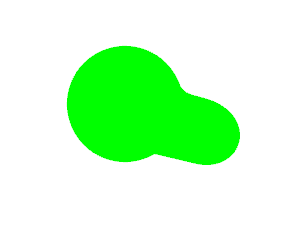
\includegraphics[width=1.5in]{figures/blend2d.png}
  \caption{Two-dimensional blend of two circles.}
\end{figure}

Adding constructive solid geometry (CSG) operations would also be useful
for modelling more advanced structures.  CSG combines primitives like 
spheres and cylinders by using the boolean set operations union,
intersection and difference.

\bibliographystyle{acmsiggraph}
\bibliography{ImplicitSurfacesRayTracer}
\end{document}

